\section{Literature Review}
\begin{frame}
	\frametitle{Literature Review}
	\framesubtitle{Table of Contents}
	{
		\hypersetup{hidelinks}
		\tableofcontents[currentsection, hideothersubsections]
	}
\end{frame}

\subsection{Milestones}
\begin{frame}
	\frametitle{Literature Review}
	\framesubtitle{Milestones}

	\begin{itemize}
		\item <1->Detection
		      \only<2>{
			      \begin{itemize}
				      \item (Faster) R-CNN~\cite{Girshick14,Girshick15,Ren17}
				      \item YOLO~\cite{Redmon15}
				      \item SSD~\cite{Liu16}
				      \item ...
			      \end{itemize}
		      }
		      \vspace{5pt}
		\item <3->Feature Extraction
		      \only<4>{
			      \begin{itemize}
				      \item Scale-Invariant Feature Transform (SIFT)~\cite{Lowe04}
				      \item Histogram of Oriented Gradients (HOG)~\cite{Dalal05}
				      \item CNNs~\cite{Lecun98}
				      \item ...
			      \end{itemize}
		      }
		      \vspace{5pt}
		\item <5->Data Association
		      \only<6>{
			      \begin{itemize}
				      \item Hungarian Algorithm~\cite{Kuhn55}
				      \item Joint Probabilistic Data Association Filters (JPDAF)~\cite{Fortmann83}
				      \item Probabilistic Occupancy Map (POM)~\cite{Fleuret08}
				      \item RNNs~\cite{Rumelhart86}
				      \item ...
			      \end{itemize}
		      }
		      \vspace{5pt}
		\item <7->Tracking
		      \only<8>{
			      \begin{itemize}
				      \item Kalman Filter~\cite{Kalman60}
				      \item Multiple Hypothesis Tracking (MHT)~\cite{Blackman04}
				      \item ...
			      \end{itemize}
		      }
		      \vspace{5pt}
		\item <9->Datasets and Challenges
		      \only<10>{
			      \begin{itemize}
				      \item see Table~\ref{tab:overview_datasets}
			      \end{itemize}
		      }
	\end{itemize}
\end{frame}

\subsubsection{Datasets and Challenges}
\begin{frame}
	\frametitle{Literature Review}
	\framesubtitle{Milestones - Datasets and Challenges}

	\begin{table}[ht]
		\centering
		\caption{Overview of Datasets}\label{tab:overview_datasets}
		\resizebox{\textwidth}{!}{
			\begin{tabular}{|l|c|c|c|c|c|c|c|c|}
				\hline
				\textbf{Dataset}                       & \textbf{Environment} & \textbf{Num. of Scenarios} & \textbf{Num. of Cameras (Overlap)} & \textbf{FPS} & \textbf{IDs} & \textbf{Year} & \textbf{Class}  \\
				\hline
				PETS~\cite{Ferryman09}                 & Outdoor              & 3                          & 8 (\cmark)                         & 25           & ---          & 2009          & Person          \\
				MARS~\cite{Zheng16b}                   & Mixed                & Multiple                   & 6 (\cmark)                         & ---          & 1261         & 2016          & Person          \\
				MOT16~\cite{Milan16a}                  & Outdoor              & 14                         & 1                                  & 25-30        & ---          & 2016          & Person, Vehicle \\
				\textbf{DukeMTMC}~\cite{Ristani16}     & Outdoor              & 1                          & 8 (\cmark)                         & 60           & 2834         & 2016          & Person          \\
				MOT17~\cite{Milan16a}                  & Outdoor              & 14                         & 1                                  & 25-30        & ---          & 2018          & Person          \\
				\textbf{Wildtrack}~\cite{Chavdarova18} & Outdoor              & Multiple                   & 7 (\cmark)                         & 2            & 313          & 2018          & Person          \\
				MSMT17~\cite{Wei18}                    & Mixed                & 12                         & 15 (\cmark)                        & 15           & 4101         & 2018          & Person          \\
				\textbf{CityFlowV1}~\cite{Tang19}      & Outdoor              & 5                          & 40 (\cmark)                        & 10           & 666          & 2019          & Vehicle         \\
				MOT20~\cite{Dendorfer20}               & Outdoor              & 8                          & 1                                  & 25           & ---          & 2020          & Person, Vehicle \\
				\textbf{CityFlowV2}~\cite{Tang19}      & Outdoor              & 6                          & 46 (\cmark)                        & 10           & 880          & 2021          & Vehicle         \\
				MMPTRACK~\cite{Han23}                  & Indoor               & 5                          & 23 (\cmark)                        & 15           & ---          & 2023          & Person          \\
				MEVID~\cite{Davila23}                  & Mixed                & 17                         & 33 (\cmark)                        & ---          & 158          & 2023          & Person          \\
				\hline
			\end{tabular}
		}
	\end{table}

	\only<2->{
		\centering
		Challenges:
		\begin{itemize}
			\centering
			\item MOT~\cite{Milan16a,Dendorfer20}
			\item AICity~\cite{Naphade23}
			\item VOT(S)~\cite{Kristan22,Kristan23}
			\item ...
		\end{itemize}
	}
\end{frame}

\begin{frame}
	\frametitle{Literature Review}
	\framesubtitle{Milestones - Datasets and Challenges}

	\begin{figure}[ht]
		\centering
		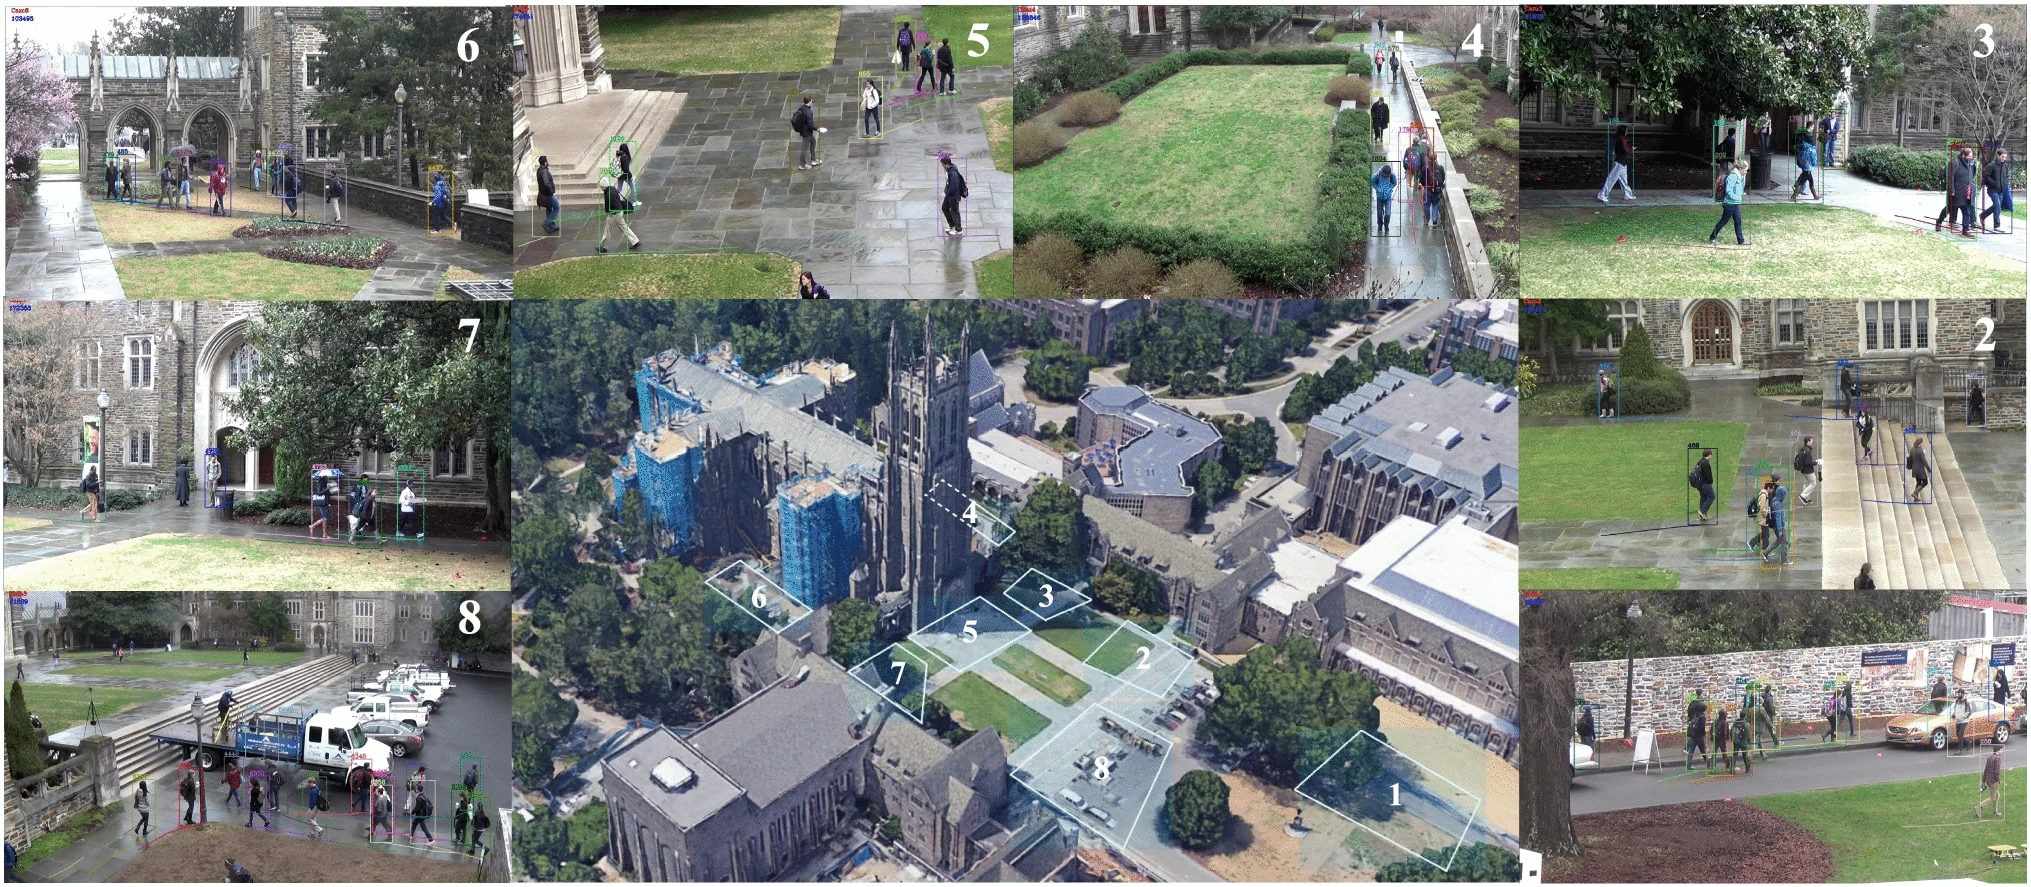
\includegraphics[width=0.75\textwidth]{resources/fig/Ma21-dukemtmc.png}
		\caption[DukeMTMC]{DukeMTMC~\cite[Fig.~2]{Ma21}}\label{fig:dukemtmc}
	\end{figure}
\end{frame}

\subsection{Tracking Paradigms}
\begin{frame}
	\frametitle{Literature Review}
	\framesubtitle{Tracking Paradigms}

	\begin{itemize}
		\item <1->\textbf{Tracking-by-Detection}
		      \only<6->{
			      \begin{itemize}
				      \item Sort~\cite{Bewley16}
				      \item DeepSORT~\cite{Wojke17}
			      \end{itemize}
		      }
		      \vspace{5pt}
		\item <2->Tracking-by-Regression
		      \vspace{5pt}
		\item <3->Tracking-by-Segmentation
		      \vspace{5pt}
		\item <4->Tracking-by-Attention
		      \vspace{5pt}
		\item <5->\textbf{Single-Shot Approaches}
		      \only<7->{
			      \begin{itemize}
				      \item Tracktor~\cite{Bergmann19}
				      \item Single-Shot Multi-Object Tracking (SMOT)~\cite{Li20}
				      \item Joint Detection and Embedding (JDE)~\cite{Wang20a}
				      \item FairMOT~\cite{Zhang21}
			      \end{itemize}
		      }
		      \vspace{10pt}
		\item[]<8->\textbf{Note:} Only refers to detection and intra-camera tracking\\(inter-camera tracking requires additional step)
	\end{itemize}
\end{frame}

\subsection{Graph-Based}
\begin{frame}
	\frametitle{Literature Review}
	\framesubtitle{Graph-Based}

	\begin{itemize}
		\item <1->Data association problem as graph
		      \vspace{5pt}
		\item <2->Nodes represent detections
		      \vspace{5pt}
		\item <3->Edges represent association costs
		      \vspace{5pt}
		\item <4->Recently use of Graph Neural Networks (GNNs)~\cite{Scarselli09}
		      \vspace{5pt}
	\end{itemize}
\end{frame}

\subsection{Edge-Computing}
\begin{frame}
	\frametitle{Literature Review}
	\framesubtitle{Edge-Computing}

	\begin{itemize}
		\item <1->\textbf{Advantages:}
		      \begin{itemize}
			      \item Process data near source
			      \item Reduce latency and bandwidth
			      \item Improve security and privacy (data not stored)
		      \end{itemize}
		      \vspace{5pt}
		\item <2->\textbf{Drawback:} Limited resources
		      \vspace{10pt}
		\item <3->\textbf{Examples:}
		      \begin{itemize}
			      \item Multi-Camera TrackingChain (MCTChain)~\cite{Wang23b}
			      \item Multi-Camera Tracking using\\Edge-Computing and Low-Power Communication~\cite{Nikodem20}
		      \end{itemize}
	\end{itemize}
\end{frame}

\subsection{Online and Real-Time}
\begin{frame}
	\frametitle{Literature Review}
	\framesubtitle{Online and Real-Time}

	\begin{itemize}
		\item <1->\citetitle{Wang21}~\cite{Wang21}
		      \begin{itemize}
			      \item Simulate checkout-free store
			      \item Fisheye cameras
			      \item Enter and exit store by scanning QR code
			      \item POM for data association
			      \item About 10 FPS without GPU
		      \end{itemize}
		      \vspace{5pt}
		\item <2->Fast-Constrained Dominant Set Clustering (FCDSC)~\cite{Tesfaye19}
		      \begin{itemize}
			      \item Graph-based approach
			      \item Consider only a sub-graph at each step
			      \item Solve intra- and inter-camera tracking simultaneously
			      \item About 18 FPS
		      \end{itemize}
	\end{itemize}
\end{frame}

\subsection{State-of-the-Art}
\begin{frame}
	\frametitle{Literature Review}
	\framesubtitle{State-of-the-Art}

	\begin{itemize}
		\item <1-> Self-supervised Camera Link Model (SCLM)~\cite{Hsu22}
		      \begin{itemize}
			      \item Graph Auto-Encoder (GAE)~\cite{Kipf16}
			      \item Zone generation algorithm
			      \item State-of-the-art on CityFlow 2019 and 2020
		      \end{itemize}
		      \vspace{5pt}
		\item <2-> Lifted Multicut Meets Geometry Projections (LMGP)~\cite{Nguyen22a}
		      \begin{itemize}
			      \item Use of POM
			      \item Bottom center of bounding box projection
			      \item State-of-the-art on Wildtrack
		      \end{itemize}
		      \vspace{5pt}
		\item <3-> EarlyBird~\cite{Teepe23}
		      \begin{itemize}
			      \item Early fusion in bird's eye view
			      \item Encoder network
			      \item Projection onto ground plane
			      \item Second best on Wildtrack
		      \end{itemize}
		      \vspace{5pt}
		\item <4-> AOT, DeAOT, DMAOT~\cite{Yang21, Yang22b}
		      \begin{itemize}
			      \item Transformer architecture
			      \item Segmentation-based tracking
			      \item Winner of VOTS2023 challenge
		      \end{itemize}
	\end{itemize}
\end{frame}

\subsection{Honorable Mentions}
\begin{frame}
	\frametitle{Literature Review}
	\framesubtitle{Honorable Mentions}

	\begin{itemize}
		\item <1->Harry Potter's Marauder's Map~\cite{Yu13}
		      \begin{itemize}
			      \item Draws parallels to Marauder's Map from Harry Potter
			      \item Localizes and tracks people
			      \item Uses color information and face recognition
			      \item Real-world nursing home, 15 cameras
		      \end{itemize}
		      \vspace{5pt}
		\item <2->MTA Dataset~\cite{Koehl20}
		      \begin{itemize}
			      \item MTMCT dataset
			      \item Virtual environment (GTA V)
			      \item Innovative approach
			      \item No privacy concerns
		      \end{itemize}
	\end{itemize}
\end{frame}